\documentclass[10pt,a4paper]{article}
\usepackage[utf8]{inputenc}
\usepackage{amsmath}
\usepackage{amsfonts}
\usepackage{amssymb}
\usepackage{graphicx}
\usepackage[swedish]{babel}
\usepackage[utf8]{inputenc}
\usepackage{amsmath}

\graphicspath{}

\author{
  \texttt{Sebastian Bångerius}
  \and
  \texttt{Andreas Nordberg}
  \and
  \texttt{Villiam Rydfalk}
  \and
  \texttt{Anton Silfver}
}

\begin{document}
\pagenumbering{gobble}

\title{Studsmatta}
\maketitle

\cleardoublepage

\tableofcontents

\clearpage

\section{Inledning}
\pagenumbering{arabic}
\setcounter{page}{3}

I den här rapporten kommer vi beskriva hur en studsmatta kan beskrivas som ett idealiserat linjärt svängningssystem av andra ordningen när en person sätter mattan i rörelse. Inom det här systemet är det personens muskelkraft som fungerar som insignalen, vilket resulterar en utsignal som alltså är studsmattans lägesändring ifrån sitt jämviktsläge. Genom att beskriva systemet med en differentialekvation av andra graden kan vi bl.a. hitta annan information om systemet, så som egenskaper om dess beteende och vilka faktorer som kan inverka på utsignalen, eller i någon mening hur svängningen påverkas av olika faktorer.

\subsection{Syfte}
Syftet med den här rapporten är att utöka vår förståelse för hur linjära system fungerar och för att få en uppfattning om hur den teorin vi lärt oss kan tillämpas i praktiken. Den här förståelsen hoppas vi alltså få ifrån vår analys av studsmattan.

\subsection{Mål}
Målet med vår rapport är att förstå hur ett linjärt system kan fungera och påverkas, alltså hur insignalen till systemet kan ändras för att få utsignalen att bete sig på ett visst sätt. Ett exempel är hur insignalen kan påverkas för att få största möjliga utsignal, med andra ord att kunna hoppa så högt som möjligt på en studsmatta.

\section{Bakgrund}

Vi har i denna rapport valt att modellera en person som hoppar på en studsmatta som en LTI (linjärt tidsinvariant) system för att undersöka dess egenskaper. Vi valde studsmattan som ett linjärt system för att analysera dess egenskaper, men även för att få en mycket verklighetsanknuten modell som inte kräver så mycket idealisering för att kunna representeras som ett linjärt svängningssystem.
\newpage

\subsection{Linjärt system}

Om vi antar att vi har ett system har insignal $x(t)$ och utsignal $y(t)$ så är vanlig notation att beteckna systemet med $x(t) \rightarrow y(t)$. Detta system kan ha flera egenskaper, men en vanlig egenskap som vi kännetecknar vårt svängande system är linjäritet. För att ett system ska vara linjärt måste det uppfylla två krav. Systemet måste dels vara additivt, d.v.s. uppfylla ekvationen
\begin{equation}
a \cdot x(t) \rightarrow a \cdot y(t) 
\end{equation}
Systemet måste också vara homogent, d.v.s. uppfylla ekvationen
\begin{equation}
x(t) = x_1(t) + x_2(t) \rightarrow y(t) = y_1(t) + y_2(t)
\end{equation}
Om man slår ihop ekvation 1 och 2 så kan man förkorta kravet till en ekvation
\begin{equation}
x(t) = a \cdot x_1(t) + b \cdot x_2(t)\rightarrow y(t) = a \cdot y_1(t) + b \cdot y_2(t)
\end{equation}
\linebreak
Således måste alla linjära system uppfylla ekvation 3 \cite{sune2000}.
I vårt system betyder detta t.ex. att en speciellt stark kraft inte kommer förstöra fjädrarna.

%[Varför är vårt system linjärt? varför är det relevant och vilka konkreta egenskaper hos linjära system använder vi oss av]

\subsection{Tidsinvarians}

%[Text om tidsinvarians]
%[ekvation?]
%[Förklaring av ekvation?]

Ett system med insignal $x(t)$ och utsignal $y(t)$ sägs vara tidsinvariant om insignalen $x(t - \tau)$ ger upphov till utsignalen $y(t - \tau)$ \cite{sune2000}. Detta betyder alltså att de fysikaliska komponenterna i systemet inte varierar över tid. I vårt fall betyder det t.ex. att våra fjädrar inte slits ut och att personen som gungar inte byter plats på mattan. 

\newpage
\section{Vårt LTI system}

\begin{figure}[ht]
\begin{center}
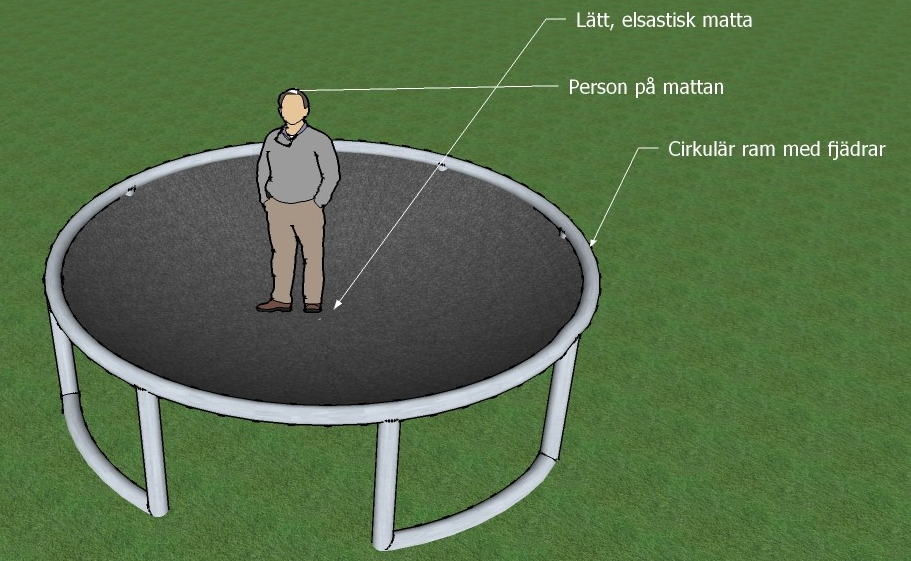
\includegraphics[scale=0.62]{Bild2}
\caption{En enkel bild av vårt system}
\end{center}
\end{figure}

Figur 1 ger en mycket enkel överblick av vårt system. Studsmattan är helt cirkulär och har fjädrar som sitter radiellt från kanten riktade in mot mitten symmetriskt runt om hela cirkeln. Vi gör antagandet att personen som hoppar står precis i mattans mitt med fötterna tätt ihop. Mattan är fäst vid personens fötter, så i själva verket hoppar hen inte utan gungar bara upp och ned genom att böja på benen.

\subsection{Idealisering}
För att inte behöva räkna på varje individuell fjäder har vi valt att modellera systemet som en enkel fjäder riktad vinkelrät mot markytan. Varför vi kan göra detta redovisas nedan:

\begin{figure}[ht]
\begin{center}
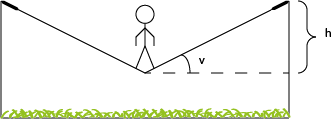
\includegraphics[scale=0.8]{fransidan}
\caption{En genomskärning från sidan}
\end{center}
\end{figure}
I figuren ses höjden $h$ samt vinkeln $v$. $h$ representerar höjdskilnaden från läget då mattan är helt platt. $v$ är vinkeln på fjädern med avseende på nyss nämnda läge.
I och med att det för varje fjäder sitter en annan fjäder på motsatt sida studsmattan (enligt figur 3) kan vi modellera fjäderkrafterna som i figur 4.
\begin{figure}[ht]
\begin{center}
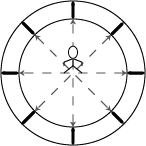
\includegraphics[scale=1]{ovanifran}
\caption{Vi ser hur det för varje fjäder finns ytterligare en, på motsatt sida}
\end{center}
\end{figure}

Vi tar nu en titt på de krafter som orsakas av ett fjäderpar ($F_1,F_2$). Dessa fjäderkrafter kan delas upp i komposanter:
\begin{figure}[ht]
\begin{center}
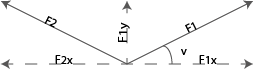
\includegraphics[scale=1]{krafter}
\caption{redovisning av krafter}
\end{center}
\end{figure}

Förutsatt att dessa fjädrar har samma fjäderkonstant och i sitt grundutförande är lika långa får vi sambanden:
$$F_1=k\Delta l_1\hat{f_1}, F_2=k\Delta l_2\hat{f_2}$$
Om nu $|\Delta l_1|=|\Delta l_2|$ kan vi konstatera att
$$F_{1x}=-F_{2x}, F_{1y}=F_{2y}$$
$$F_{tot}=F_1+F_2=(F_{1y}+F_{2y})\hat{y}=2k\Delta l\sin(v)\hat{y}$$

\pagebreak
Vi tar nu en titt på figur 5 som beskriver fjäderns utsträckning. Detta för att kunna uttrycka kraften som en funktion av $h$ och $k$ istället för $l$ och $k$.

\begin{figure}[ht]
\begin{center}
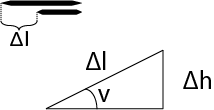
\includegraphics[scale=0.5]{utstrackning}
\caption{Utsträckning för en fjäder}
\end{center}
\end{figure}

$$\Delta h = \Delta l \sin(v) \rightarrow F_{tot}=2k\Delta l \sin(v)=2k\Delta h\propto k\Delta h $$

\begin{figure}[ht]
\begin{center}
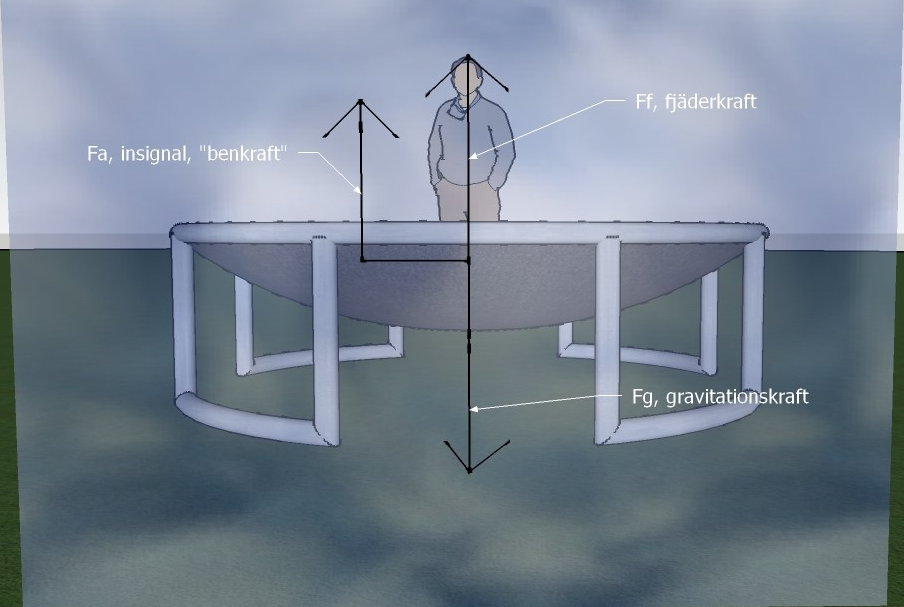
\includegraphics[scale=0.5]{BildKrafter}
\caption{Utsträckning för en fjäder}
\end{center}
\end{figure}

Vi kan alltså modellera vår studsmatta som en enkel fjäder som står på marken under den "gungande" personens fötter.
Insignalen i vårt system blir alltså kraften som den hoppande personen utför på systemet då denne böjer eller sträcker på benen. Utsignalen i systemet definieras som mattans ändring i höjdled med referenspunkt i jämviktsläget på studsmattan. 
%Jämviktsläget varierar i höjd beroende på massan som står på mattan.
%Uppdatera till att matcha den slutliga referensbilden
Krafterna uttryckta med pilar i figur 1 är gravitationskraften från massan $F_g$, fjäderns motkraft på massan $F_f$ och kraften från personen som trycker emot $F_a$.

Då fjädrarna i vår studsmatta är placerade symmetriskt och personen står placerad i mitten av mattan kan vi idealisera systemet som en enda fjäder verkande i y-led, eftersom de radiella krafterna tar ut varandra i symmetrin.

\subsection{Gravitationskraften $F_g$}

\begin{equation}
F_g = m \cdot g
\end{equation}
Gravitationskraften $F_g$ är den kraften som påverkar en massa $m$ med en konstant gravitationsacceleration $g$.

\subsection{Fjäderkraften $F_f$}

Fjäderkraften $F_f$ är den kraft som motverkar en fjäders avskiljning ifrån sitt jämviktsläge. Sambandet har namnet Hookes lag. Om fjäderns grundjämviktsläge är $L$ och dess jämviktsläge efter att massan läggs på är $l_1$ så kan vi uttrycka avvikelsen från jämviktsläget vid $t=0$ som $l_0 = L - l_1$. Eftersom vi har avvikelsen från jämviktsläget $l_1$ så lägger vi på $y(t)$. Fjäderkonstanten sätts till $k$. Denna kraft är motriktad den av gravitationen och uttrycks på följande vis:

\begin{equation}
F_f = -k (l_0 + y(t))
\end{equation}

\subsection{Dämpningskraften $F_d$}
\begin{equation}
F_d = -c \cdot v
\end{equation}
Dämpningskraften $F_d$ är den kraft som motverkar rörelsen i ett svängningssystem där $v$ är objektet i rörelses momentana hastighet och $c$ är dämpningskoefficienten för svängningsrörelsen. Denna kraft är motriktad den av gravitationen.

\subsection{Slutgiltig differentialekvation}

Systemet består av de åvanstående tre krafterna samt insignalen som alla är krafter i y-led. Summan av dessa krafter skapar den totala kraften $F_{tot}$. Vi kan då beskriva vårt system med följande ekvation.

\begin{equation}
F_{tot} = F_a + F_g + F_f + F_d
\end{equation}

Vi sätter $F_a$ som insignalen $x(t)$ vilket tillsammans med våra tidigare definitioner och Newtons lag ger:

\begin{equation}
F_{tot} = x(t) + mg - k(l_0+y(t)) - cv = ma
\end{equation}

Vi uttrycker hastighet och acceleration som funktioner av t.
\begin{equation}
a = \frac{d^2y(t)}{dt^2} , v = \frac{y(t)}{dt}
\end{equation}

Vilket ger:

\begin{equation}
 m\frac{d^2y(t)}{dt^2} =  -k(l_0 + y(t)) -c\frac{dy(t)}{dt} + mg +  x(t)
\end{equation}

Vid $t = 0$ så kommer 
\begin{equation}
k \cdot l_0 = mg
\end{equation}

Vilket ger vår slutgiltiga differentialekvation.
\begin{equation}
 m\frac{d^2y(t)}{dt^2} + k \cdot y(t)) + c\frac{dy(t)}{dt} = x(t)
\end{equation}

\subsection{Linjäritetsbevis}

För att visa att vårt system är linjärt måste vi visa att det är både homogent och additivt som tidigare nämnt. Om vi antar att insignalen $x_1(t) \rightarrow y_1(t)$ och $x_2(t) \rightarrow y_2(t)$ så gäller att:

\begin{equation}
m\frac{d^2y_1(t)}{dt^2} + c\frac{dy_1(t)}{dt} + ky_1(t) = x_1(t)
\end{equation}

\begin{equation}
m\frac{d^2y_2(t)}{dt^2} + c\frac{dy_2(t)}{dt} + ky_2(t) = x_2(t)
\end{equation}


Om vi då låter insignalen vara $a_1 x_1(t) + a_2 x_2(t)$ där $a_1$ och $a_2$ är reella konstanter så ger det:
\begin{equation}
m\frac{d^2y(t)}{dt^2} + c\frac{dy(t)}{dt} + ky(t) = a_1 x_1(t) + a_2 x_2(t)
\end{equation}

Ekvation 9 och 10 ger:

\begin{multline}
m\frac{d^2y(t)}{dt^2} + c\frac{dy(t)}{dt} + ky(t) = \\ a_1(m\frac{d^2y_1(t)}{dt^2} + c\frac{dy_1(t)}{dt} + ky_1(t)) + a_2(m\frac{d^2y_2(t)}{dt^2} + c\frac{dy_2(t)}{dt} + ky_2(t))
\end{multline}

Högerledet i ekvation 12 kan skrivas:

\begin{equation}
m\frac{d^2\{a_1y_1(t) + a_2y_2(t)\}}{dt^2} + c\frac{d\{a_1y_1(t) + a_2y_2(t)\}}{dt} + k\{a_1y_1(t) + a_2y_2(t)\}
\end{equation}

Vilket ger:
\begin{multline}
m\frac{d^2y(t)}{dt^2} + cm\frac{dy(t)}{dt} + ky(t) = \\ m\frac{d^2\{a_1y_1(t) + a_2y_2(t)\}}{dt^2} + c\frac{d\{a_1y_1(t) + a_2y_2(t)\}}{dt} + k\{a_1y_1(t) + a_2y_2(t)\}
\end{multline}

Alltså:

\begin{equation}
y(t) = a_1 y_1(t) + a_2 y_2(t)
\end{equation}

Systemet uppfyller således kravet för linjäritet.

\subsection{Systemfunktionen}

Från differentialekvationen kan vi genom laplacetransformering ta fram systemfunktionen $H(s)$.

\begin{multline}
 m\frac{d^2y(t)}{dt^2} + k \cdot y(t) + c\frac{dy(t)}{dt} = x(t) \\ \leftrightarrow m \cdot s^2 \cdot Y(s) + c \cdot s \cdot Y(s) + k \cdot Y(s) = X(s)
\end{multline}

Bryter vi ut $Y(s)$ i vänsterledet får vi:

\begin{equation}
Y(s)(m \cdot s^2 + c \cdot s + k) = X(s)
\end{equation}

Eftersom $H(s) = \frac{Y(s)}{X(s)}$ så flyttar vi om och får:

\begin{equation}
H(s) = \frac{Y(s)}{X(s)} = \frac{1}{m\cdot s^2 + c \cdot s + k}
\end{equation}

Om vi tar fram rötterna till nämnaren får vi:

\begin{equation}
H(s)= \frac{1}{(s + \frac{c}{2 \cdot m} + \sqrt{ (\frac{c}{2 \cdot m})^2 - \frac{k}{m}}) (s + \frac{c}{2 \cdot m} - \sqrt{ (\frac{c}{2 \cdot m})^2 - \frac{k}{m}})}
\end{equation}

Poler produceras där nämnarpolynomet har sina rötter.

\begin{equation}
S_{rot}=-\frac{c}{2m} \pm \sqrt{(\frac{c}{2m})^2-\frac{k}{m}}
\end{equation}

Vi ser att vi antingen kan få två komplexa rötter, en reell dubbelrot, eller två reella rötter. Vi har alltså tre distinkt olika sätt som våra poler kan placera sig på enligt följande:
\begin{itemize}

\item $H(s)$ har en dubbelrot om $\sqrt{(\frac{c}{2m})^2-\frac{k}{m}}=0$ (Då är $S_{rot}=-\frac{c}{2m}$)


\item $H(s)$ har två rella rötter om $0\neq\sqrt{(\frac{c}{2m})^2-\frac{k}{m}}\in \mathbb{R}$ \newline d.v.s. om $(\frac{c}{2m})^2-\frac{k}{m}>0$


\item $H(s)$ har två komplexa rötter om $\sqrt{(\frac{c}{2m})^2-\frac{k}{m}}\notin \mathbb{R}$ \newline d.v.s. om $(\frac{c}{2m})^2-\frac{k}{m}<0$



\end{itemize}

Detta kan förenklas till

\begin{itemize}
\item Dubbelpol $S_{rot}=-\frac{c}{2m}$ om $k=\frac{c^2}{4m}$
\begin{center}
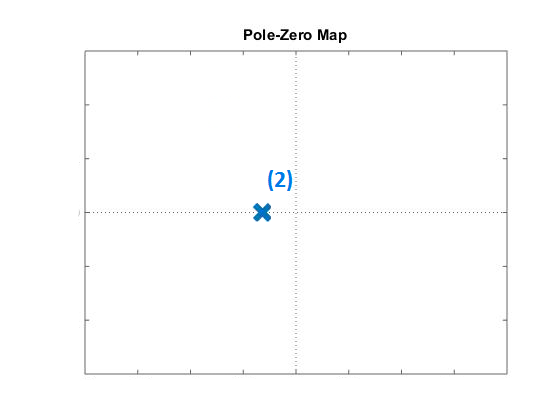
\includegraphics[scale=0.3]{1reell}
\end{center}
\item Två reella poler om $k<\frac{c^2}{4m}$
\begin{center}
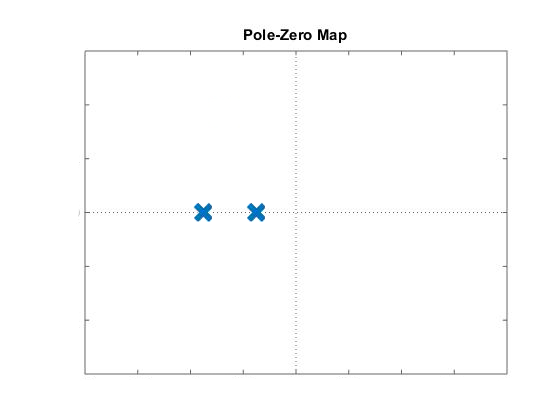
\includegraphics[scale=0.3]{2reella}
\end{center}
\item Två komplexa poler om $k>\frac{c^2}{4m}$
\begin{center}
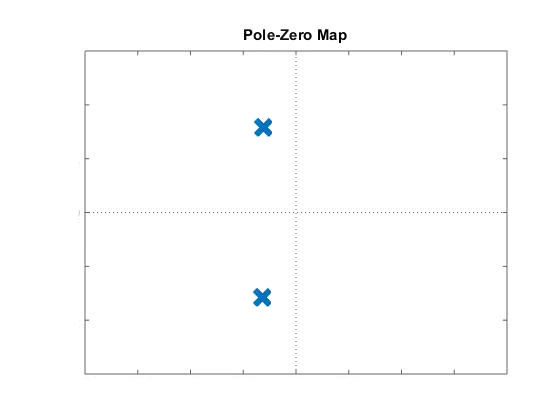
\includegraphics[scale=0.3]{2komplexa}
\end{center}
\end{itemize}

I vårt fall (studsmatta) vill vi gärna skapa så hög amplitud ut som möjligt. Mycket svängning och lite dämpning. Detta återfinns i det tredje fallet (två komplexa rötter) och brukar kallas för ett underdämpat system. Detta visualiseras grafiskt i form av ett amplitudspektrum i figur XXX. Nedan ses ett pol/nollställe-diagram över vårt system med följande konstanter insatta $k=1000\frac{N}{m}$ , $m=70kg$ , $c=100\frac{kg}{s}$.

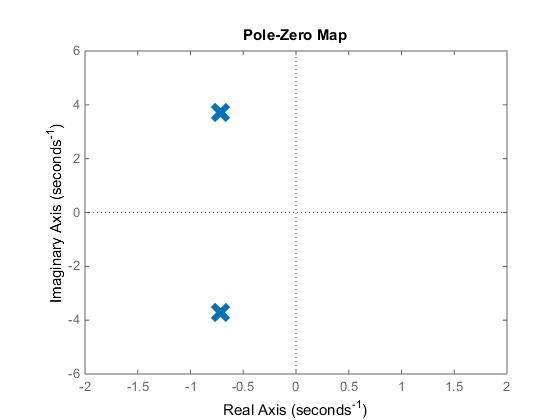
\includegraphics[scale=0.5]{nolpol-diagram}

\subsection{Impulssvar}

Genom att kvadratkomplettera $H(s)$ får vi:

\begin{equation}
H(s) = \frac{1}{m} \cdot \frac{1}{(s+(\frac{c}{2 \cdot m}))^2-(\frac{c}{2 \cdot m})^2+\frac{k}{m}} 
\end{equation}

Om vi sätter $\alpha = \frac{c}{2m}$ och $\omega_0^2 = {-\frac{c + 4\cdot k \cdot m^2}{4 \cdot m^2}}$ och multiplicerar med $\frac{\omega_0}{\omega_0}$ får vi:

\begin{equation}
H(s) = \frac{1}{\omega_0 \cdot m} \cdot \frac{\omega_0}{(s + \alpha)^2 +\omega_0^2}
\end{equation}

Genom att inverslaplacetransformera $H(s)$ får vi impulssvaret $h(t)$. Vi använder tabell 19.23 i Sune Söderkvist formelsamling:

\begin{multline}
h(t) = \frac{1}{\omega_0 \cdot m} \cdot e^{-\alpha \cdot t} \cdot sin(\omega_0 \cdot t) \cdot u(t) = \\ \frac{1}{\sqrt{\frac{4 \cdot m \cdot k - c^2}{4}} }  \cdot e^{-\frac{c}{2m} \cdot t} \cdot sin(\sqrt{\frac{4 \cdot m \cdot k - c^2}{4 \cdot m^2}} \cdot t) \cdot u(t)
\end{multline}

\subsection{Stabilitetsbevis}
För att vår idealisering skall vara representativ för vår studsmatta måste systemet vara stabilt. I grund och botten betyder detta att vårt system måste läcka energi. Detta stämmer om vårt 


\newpage

\begin{thebibliography}{9}

\bibitem{sune2000}
  Sune Söderkvist,
  \emph{Tidskontinuerliga Signaler \& System}.
  \linebreak
  Erik Larsson AB, Linköping,
  3e upplagan,
  2000.

\end{thebibliography}

\end{document}